\documentclass{beamer}
\usepackage[dutch]{babel}
\usepackage{amsmath}
\usepackage{fancyhdr}
\usepackage{url}
\usepackage{color}
\usepackage{graphicx}
\usepackage[latin1]{inputenc}
\usepackage{marvosym}
\usepackage{textcomp}
\usepackage{listings}
\usepackage{lipsum}
\usepackage{hyperref}
\usepackage{algorithm2e}

\input lua.sty

\definecolor{dkgreen}{rgb}{0,0.6,0}
\definecolor{gray}{rgb}{0.5,0.5,0.5}
\definecolor{mauve}{rgb}{0.58,0,0.82}

\lstset{frame=tb,
    language=lua,
    aboveskip=3mm,
    belowskip=3mm,
    showstringspaces=false,
    columns=flexible,
    captionpos=b,
    basicstyle={\small\ttfamily},
    numbers=none,
    numberstyle=\tiny\color{gray},
    keywordstyle=\color{blue},
    commentstyle=\color{dkgreen},
    stringstyle=\color{mauve},
    breaklines=true,
    breakatwhitespace=true
    tabsize=3
}

\definecolor{beamer@background}{RGB}{233,233,255}
\setbeamercolor{background canvas}{bg=beamer@background}
\definecolor{beamer@sidebarbackground}{RGB}{100,120,230}
\setbeamercolor{sidebar canvas left}{bg=beamer@sidebarbackground}

\setbeamertemplate{caption}{\insertcaption}

\usetheme[width=100pt]{Goettingen}
\begin{document}

\title{Programming in Lua}
\author{Maico Timmerman \& Robin Klusman}
\date{15 November 2013}

%Frame 1
\begin{frame}
    \maketitle
\end{frame}

% Frame 2
\begin{frame}
    \section{$ \Rightarrow $ History of Lua}
    \frametitle{History}
    \begin{itemize}
        \item{Released in 1993}
        \item{Computer Graphhics Technology Group}
        \item{Rio de Janeiro}
        \item{Import taxes}
        \item{Lua and SOL}
    \end{itemize}	
\end{frame}

% Frame 3
\begin{frame}
    \section{$ \Rightarrow $ What is Lua?}
    \frametitle{What is Lua?}
    \begin{itemize}
        \item{Simple object language}
        \item{Data-entry language}
        \item{Incorporates SOL and DEL syntax}
        \item{Small amount of Data Types}
        \item{Dynamically typed}
    \end{itemize}
\end{frame}

% Frame 4
\begin{frame}[fragile]
    \section{$ \Rightarrow $ Lua Syntax}
    \frametitle{Lua syntax}
    \begin{itemize}
        \item{No $\lbrace$ $\rbrace$ ; and : in default syntax}
        \item{Commenting using \texttt{--comment} for comments:}
            \begin{lstlisting}[language=lua]
--this is a comment!
function gcd(nom, den)
    ...
            \end{lstlisting}
        \item{\texttt{--[[comment]]} for multilinecomments:}
            \begin{lstlisting}[language=lua]
--[[ this is a long comment! ]]
function gcd(nom, den)
    ...
            \end{lstlisting}
        \item{bloks end with \texttt{end}}
        \begin{lstlisting}[language=lua]
function gcd(nom, den)
    ...
end
            \end{lstlisting}
\end{itemize}
\end{frame}

% Frame 5
\begin{frame}[fragile]
    \frametitle{Lua syntax}
    \begin{itemize}
        \item{local variables need to be specified:}
            \begin{lstlisting}[language=lua]
local thisVarIsLocal
            \end{lstlisting}
        \item{arrays do not exists, use tables instead:}
            \begin{lstlisting}[language=lua]
--table as array
t = { 1,2,3,5,8,13 }
print t[0] --returns nil!
print t[1] --returns 1
--table as dictionary
t = { apple="green", orange="orange" }
print t[apple] --returns "green"
            \end{lstlisting}
\end{itemize}
\end{frame}

% Frame 6
\begin{frame}[fragile]
    \section{$ \Rightarrow $ Lua coding}
    \frametitle{Lua coding - Scopes}
    \begin{lstlisting}[language=lua]
local myLocalVariable = "Hello"
function myFunction()
  local myVariable = 5
  mySecondVariable = 200
  -- ... instructions ...
end
print( myVariable ) -- Outputs: "nil"
print( mySecondVariable ) -- Outputs: "200"
print( myLocalVariable ) -- Outputs: "Hello"
    \end{lstlisting}
\end{frame}

% Frame 7
\begin{frame}[fragile]
    \frametitle{Lua coding - Control Flow}
    \begin{lstlisting}[language=lua]
for i,v in ipairs(t) do
  if type(v) == "string" then
    print(v)
  end
end
    \end{lstlisting}
\end{frame}

% Frame 8
\begin{frame}[fragile]
    \section{$ \Rightarrow $ Lua at work}
    \frametitle{Lua at work- ComputerCraft}
    \begin{figure}
        % http://www.computercraft.info/forums2/index.php?/topic/14877-panel-terminal-redirection-to-parts-of-screen/
        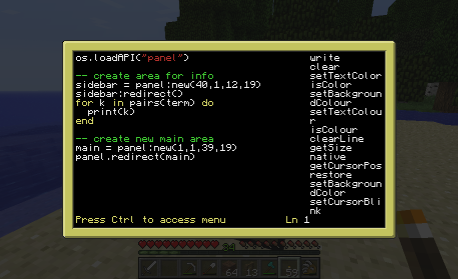
\includegraphics[width=1\textwidth]{computercraft}
        \caption{Computercraft by Dan200}
        \textit{test}
    \end{figure}
\end{frame}

% Frame 9
\begin{frame}[fragile]
    \frametitle{Lua at work - Awesome window manager}
    \begin{figure}
        % http://www.abclinuxu.cz/desktopy/asfethan-20120422
        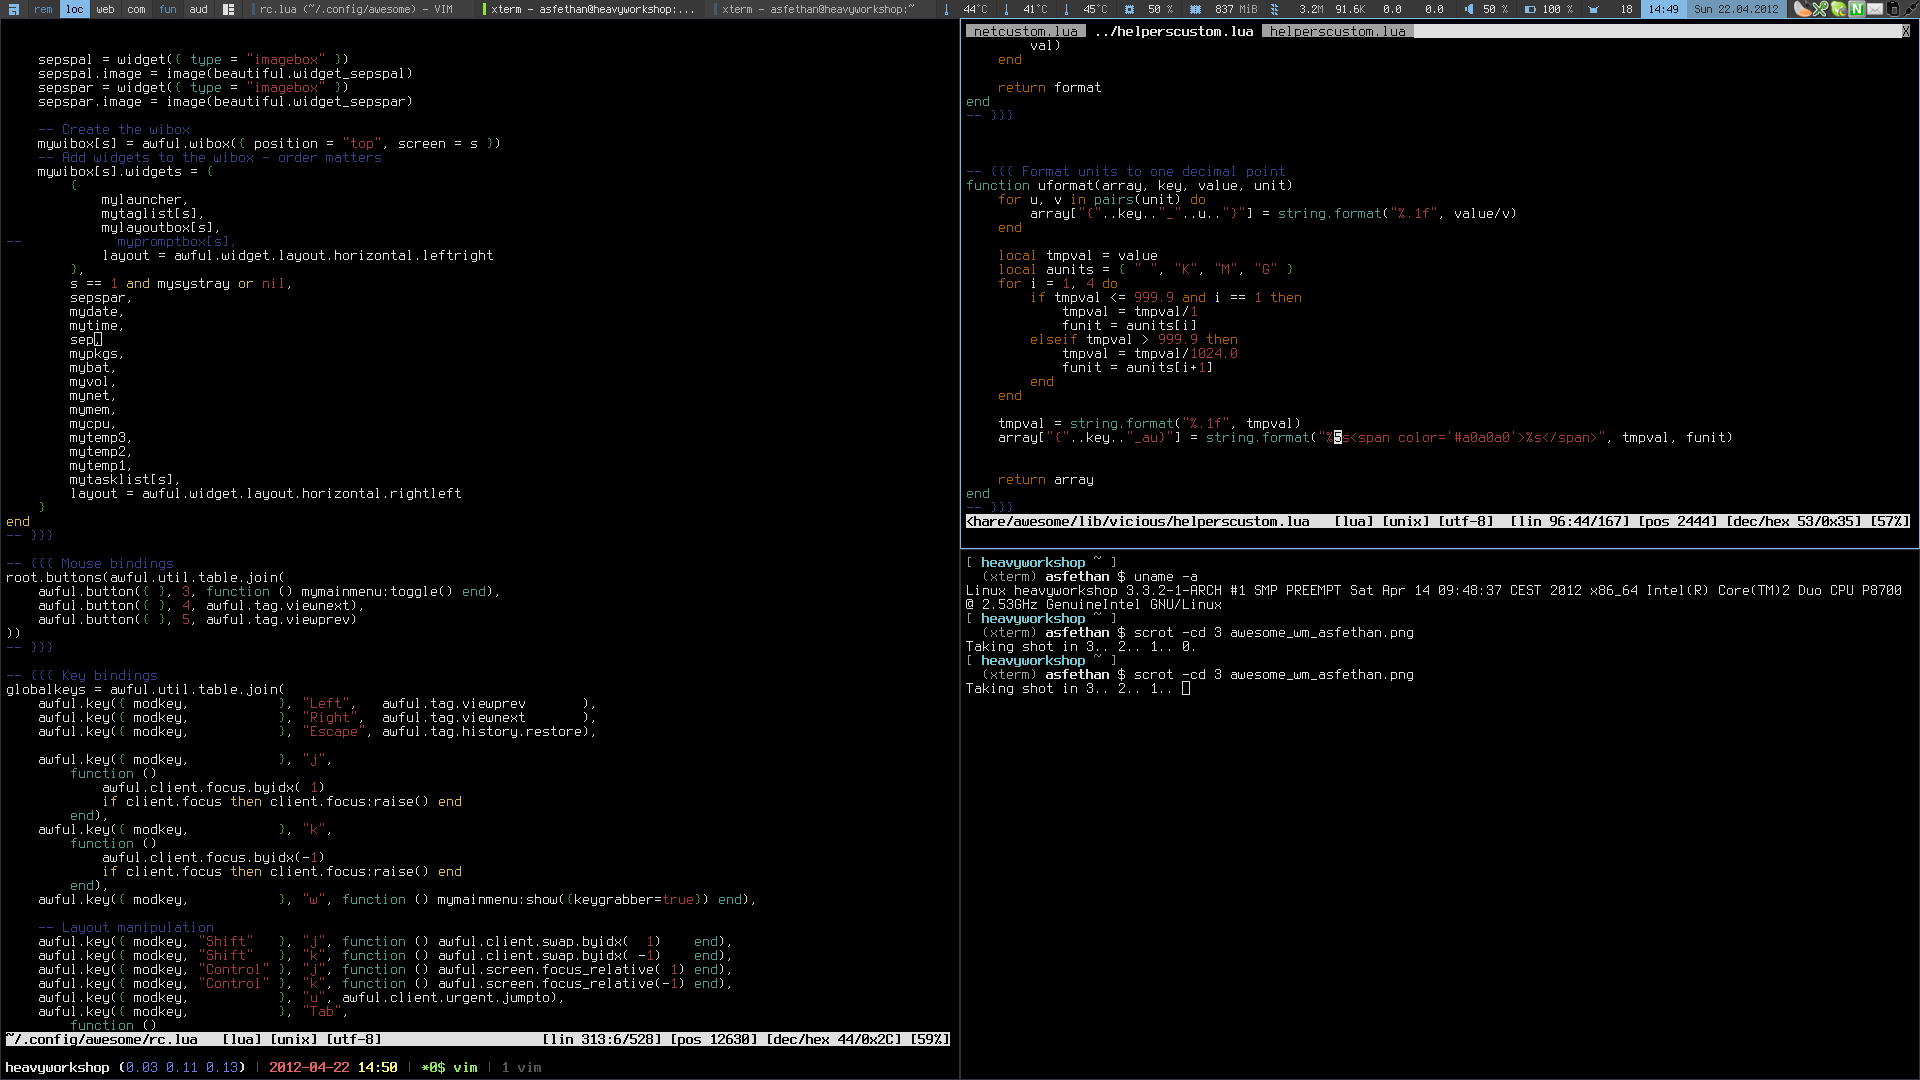
\includegraphics[width=1\textwidth]{awesomewm}
        \caption{awesomewm by Naquadah}
    \end{figure}
\end{frame}

% Frame 10
\begin{frame}[fragile]
    \frametitle{Lua at work - Games}
    \begin{figure}
        
\includegraphics[width=1\textwidth]{games}
        \caption{Games using or implementing lua.}
    \end{figure}
\end{frame}

\bgroup
    \setbeamercolor{background canvas}{bg=black}
    \begin{frame}[plain]{}
    \end{frame}
\egroup

\end{document}
